\documentclass[a4paper,12pt,openany]{book}

\usepackage[nohdr]{evan}
\usepackage{xcolor}
\usepackage{amsmath, amsfonts}
\usepackage{amssymb}
\usepackage{fancyhdr}
\usepackage{graphicx}
\usepackage{float}
%\usepackage[margin=1.0in]{geometry}

\pagestyle{fancy}

\begin{document}
	\title{MAT 251 (Numerical Method) Project\\[2\baselineskip]
	Lecturer: \textcolor{teal}{Mr. D.A Dikko} }
	\author{\Large{Group 6 (Julia)}}
	\date{}
	\maketitle
	
	\section{Abstract}
		This is the solution to the problems given on the MAT 251 projects. In this work we collaboratively worked together to solve each problems with the computer programming language called \textcolor{red}{Julia}
	%\end{abstract}
	\section{Contributors}
	In this section we give list of the names of those who contributed to the success of this work.
	
	
	\begin{tabular}{|c|c|c|}
		\hline
		Name & Matric. Number & Department \\
		\hline
		Ogunjinmi Adeshina Toheeb & 215076 & Mathematics\\
		\hline
		Victoria Ojubuyi & 215247 & Statistics\\
		\hline
		Alade George Oluwaseyi & 215659 & Statistics \\
		\hline 
		Adeniyi Taofeek & 215042 & Mathematics\\
		\hline
		Hannah Adaeze Udeala & 215097 & Mathematics \\
		\hline 
		Busari SIDIKAT Abiodun & 215057 & Mathematics \\
		\hline
		FATOKUN PEACE OLUWADEMILADE & 215065 & Mathematics \\
		\hline 
		Adeona Tosin Samuel & 215044 & Mathematics \\
		\hline
		Popoola Divine Gbolahan & 215262 & Statistics \\
		\hline 
		Kanikwu Enoch ECHEZONACHUKWU & 215243 & Statistics \\
		\hline 
		Akinwande Micheal & 215052 & Mathematics \\
		\hline
		Babatunde Adeleke Moses & 215056 & Mathematics \\
		\hline
		OSOTA Ayomikun & 215087 & Mathematics \\
		\hline
	\end{tabular}
\newpage
\tableofcontents
\newpage
\chapter{Introduction}
\section{A brief introduction to Julia}

Julia is a high-level, high-performance, dynamic programming language. While it is a general-purpose language and can be used to write any application, many of its features are well suited for numerical analysis and computational science.

Work on Julia was started in 2009, by Jeff Bezanson, Stefan Karpinski, Viral B. Shah, and Alan Edelman, who set out to create a free language that was both high-level and fast. On 14 February 2012, the team launched a website with a blog post explaining the language's mission. In an interview with InfoWorld in April 2012, Karpinski said of the name "Julia": "There's no good reason, really. It just seemed like a pretty name." Bezanson said he chose the name on the recommendation of a friend, then later wrote that Julia stands for "Jeff’s uncommon lisp is automated"

\section{Notable uses of Julia}
Julia has attracted some high-profile users, from investment manager BlackRock, which uses it for time-series analytics, to the British insurer Aviva, which uses it for risk calculations. In 2015, the Federal Reserve Bank of New York used Julia to make models of the United States economy, noting that the language made model estimation "about 10 times faster" than its previous MATLAB implementation. Julia's co-founders established Julia Computing in 2015 to provide paid support, training, and consulting services to clients, though Julia remains free to use. At the 2017 JuliaCon conference, Jeffrey Regier, Keno Fischer and others announced that the Celeste project used Julia to achieve "peak performance of 1.54 petaFLOPS using 1.3 million threads" on 9300 Knights Landing (KNL) nodes of the Cori II (Cray XC40) supercomputer (then 6th fastest computer in the world). Julia thus joins C, C++, and Fortran as high-level languages in which petaFLOPS computations have been achieved.


Three of the Julia co-creators are the recipients of the 2019 James H. Wilkinson Prize for Numerical Software (awarded every four years) "for the creation of Julia, an innovative environment for the creation of high-performance tools that enable the analysis and solution of computational science problems." Also, Alan Edelman, professor of applied mathematics at MIT, has been selected to receive the 2019 IEEE Computer Society Sidney Fernbach Award "for outstanding breakthroughs in high-performance computing, linear algebra, and computational science and for contributions to the Julia programming language."


Julia Computing and NVIDIA announce "the availability of the Julia programming language as a pre-packaged container on the NVIDIA GPU Cloud (NGC) container registry" with NVIDIA stating "Easily Deploy Julia on x86 and Arm  Julia offers a package for a comprehensive HPC ecosystem covering machine learning, data science, various scientific domains and visualization."


Additionally, "Julia was selected by the Climate Modeling Alliance as the sole implementation language for their next generation global climate model. This multi-million dollar project aims to build an earth-scale climate model providing insight into the effects and challenges of climate change."


Julia is used by NASA and the Brazilian INPE for space mission planning and satellite simulation. Another effort is working on an embedded project to control a satellite in space using Julia for attitude control.

\section{Features of Julia}
Here are some of the features Julia that makes it distinct from other languages.
\begin{enumerate}
    \item Multiple dispatch: providing ability to define function behavior across many combinations of argument types
	\item Dynamic type system: types for documentation, optimization, and dispatch
	\item Performance approaching that of statically-typed languages like C
	\item A built-in package manager
	\item Lisp-like macros and other metaprogramming facilities
	\item Call C functions directly: no wrappers or special APIs
 	\item Ability to interface with other languages, e.g. Python with PyCall,[b] R with RCall, and Java/Scala with JavaCall
	\item Powerful shell-like abilities to manage other processes
	\item Designed for parallel and distributed computing
	\item Coroutines: lightweight green threading
	\item User-defined types are as fast and compact as built-ins
	\item Automatic generation of efficient, specialized code for different argument types
	\item Elegant and extensible conversions and promotions for numeric and other types
	\item Efficient support for Unicode, including but not limited to UTF-8
\end{enumerate}

%\section{Some shortcomings of Julia}
\chapter{Solutions to Problems}
\begin{problem}[Runge-Kutta]
	Write simple code to evaluate the Runge-Kutta method.
	
	Hence solve $\frac{\rm dy}{\rm dx} = \frac{1}{x + y}$ for $x = 2.0$ with initial values $x=0,y=1$ and interval length $h = 0.1$
\end{problem}

\begin{soln}
	Below is the figure showing the code used for the computation of Runge-Kutta method
	\begin{figure}[H]
		\centering
		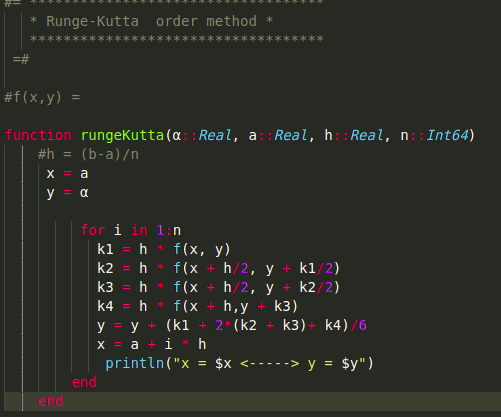
\includegraphics[width = .7\linewidth]{pic1}
		\caption{Julia code for Rnuge-Kutta method}
	\end{figure}
From the code we have \texttt{\#f(x,y) =  } this is where we input the given function.
To do this we firstly comment it out by deleting the \texttt{\#} character.

To solve the given equation in the problem we have the following

\begin{figure}[H]
	\centering
	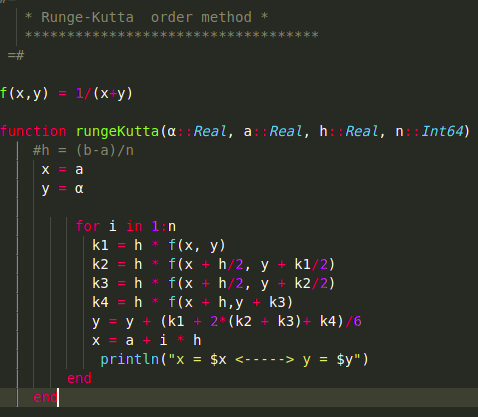
\includegraphics[width = .7\linewidth]{pic2}
	\caption{Julia code for Rnuge-Kutta method with $f = \frac{1}{x+y}$ included}
\end{figure}
Running the function, we take $\alpha = y_0 = 1,x_0 = 0, h=0.1$ and the number of values to be $n = 20$ then we have 
\begin{figure}[H]
	\centering
	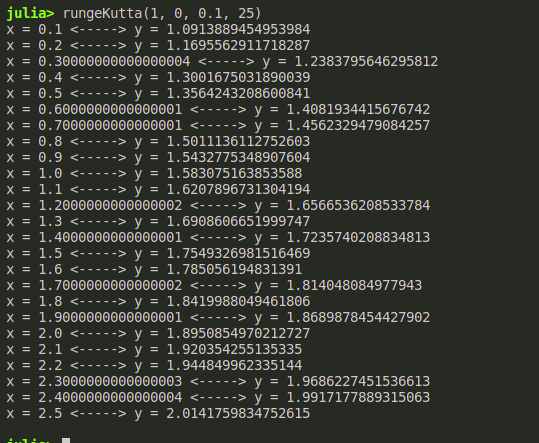
\includegraphics[width = .7\linewidth]{pic3}
	\caption{Running the Runge-Kutta code}
\end{figure}

\begin{figure}[H]
	\centering
	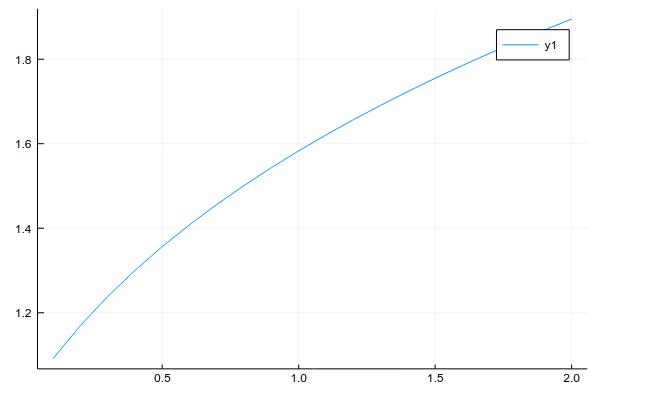
\includegraphics[width = .7\linewidth]{pic23}
	\caption{Plotting the Runge-Kutta method solution for $\frac{dy}{dx} = \frac{1}{x+y}$}
\end{figure}

\begin{tabular}{|c | c|}
	\hline
	$x$ & $y$ \\
	\hline
	0.1 & 1.0913889454953984\\
	0.2 & 1.1695562911718287\\
	0.3 & 1.2383795646295812\\
	0.4 & 1.3001675031890039\\
	0.5 & 1.3564243208600841\\
	0.6 & 1.4081934415676742\\
	0.7 & 1.4562329479084257\\
	0.8 & 1.5011136112752603\\
	0.9 & 1.5432775348907604\\
	1.0 & 1.583075163853588\\
	1.1 & 1.6207896731304194\\
	1.2 & 1.6566536208533784\\
	1.3 & 1.6908606651999747\\
	1.4 & 1.7235740208834813\\
	1.5 & 1.7549326981516469\\
	1.6 & 1.785056194831391\\
	1.7 & 1.814048084977943\\
	1.8 & 1.8419988049461806\\
	1.9 & 1.8689878454427902\\
	2.0 & 1.8950854970212727\\
	\hline
\end{tabular}


From the above figure we observe that $$\text{when } x = 2.0, \quad y \approx 1.8950854970212727$$
\end{soln}

\begin{problem}[Milne's method]
	\begin{enumerate}
		\item Write codes to represent the Milne's method.
		\item Solve numerically at $x = 0.4,0.5$ given values $x = 0,0.1,0.2,0.3$
		\item Hence solve $\frac{dy}{dx} = 2e^x - y$ given that $y_0 = 2, y_1 = 2.010, y_2 = 2.040, y_3 = 2.09$
	\end{enumerate}
\end{problem}

\begin{soln}
	The code is given in the figure below
	\begin{figure}[H]
		\centering
		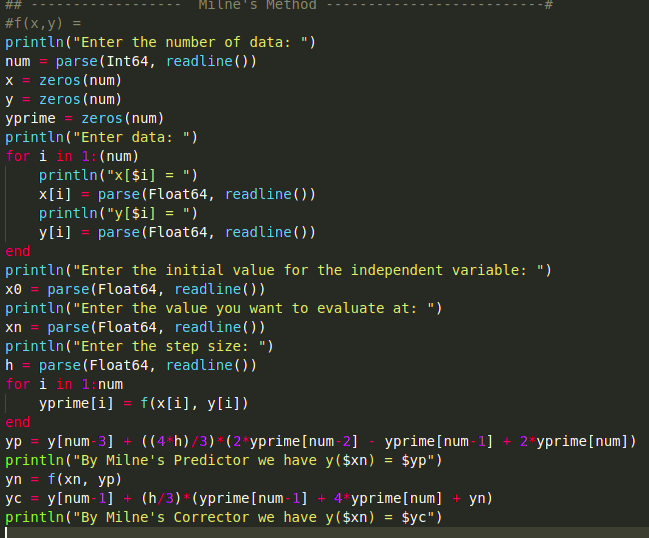
\includegraphics[width = .7\linewidth]{pic4}
		\caption{Julia code for the Milne's method}
	\end{figure}

Similarly as in problem 1 we input the values of $f = 2e^x - y$ into the code with $h = 0.1$ and the initial value of $y(0) = 2$ as shown in the figure below for $x = 0.4$
\begin{figure}[H]
	\centering
	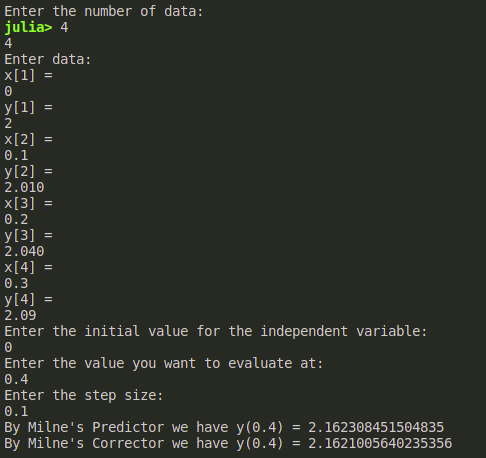
\includegraphics[width=.5\linewidth]{pic5}
	\caption{Evaluation of $\frac{dy}{dx} = 2e^x - y$ at $x = 0.4$ by Milne's method}
\end{figure}
For $x = 0.5$ we have the following
\begin{figure}[H]
	\centering
	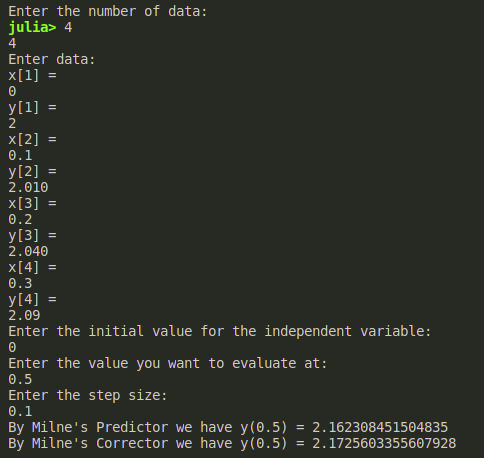
\includegraphics[width = .7\linewidth]{pic6}
	\caption{Evaluation of $\frac{dy}{dx} = 2e^x - y$ at $x = 0.5$ by Milne's method}
\end{figure}

\end{soln}

\begin{problem}[Adams bashforth-Moulton formula]
	\begin{enumerate}
		\item Write code to represent a solution of the Adams-Bashforth-Moulton predictor-corrector formula.
		\item Hence evaluate $y(1.4)$ if $y$ satisfies $\frac{dy}{dx} + \frac{y}{x} = \frac{1}{x^2}$ and $$y_{1} = 1, y_{1.1} = 0.996, y_{1.2} = 0.986, y_{1.3} = 0.972$$
	\end{enumerate}
\end{problem}

\begin{soln}
	The code for computation is given below
	\begin{figure}[H]
		\centering
		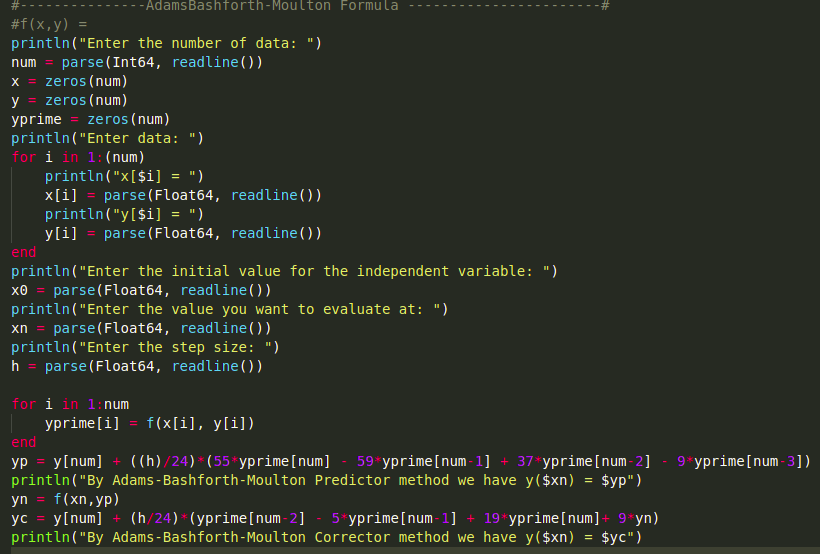
\includegraphics[width = .7\linewidth]{pic7}
		\caption{Julia code for the Adams Bashforth-Moulton formula}
	\end{figure}
Input the function and solve we have the following
\begin{figure}[H]
	\centering
	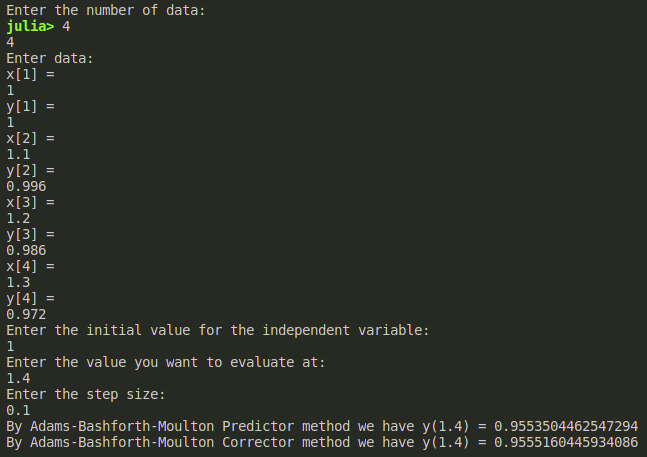
\includegraphics[width = .7\linewidth]{pic8}
	\caption{Evaluation of $\frac{dy}{dx} + \frac{y}{x} = \frac{1}{x^2}$ at $x = 1.4$ by Adams Bashforth-Moulton formula}
\end{figure}
\end{soln}

\begin{problem}[Lagrange Interpolation]
	\begin{enumerate}
		\item Using Lagrange interpolation method, write a code to represent this.\\
		Hence use the code to determine the values $f$ at $x = 2.5$ given the following table
		
		\begin{tabular}{|c|c|c|}
			\hline 
			$n$ & $x_n$ & $y_n = f(x)$ \\
			\hline
			0 & 1 & 4 \\
			1 & 2 & 14 \\
			2 & 3 & 40 \\
			3 & 4 & 88\\
			\hline
		\end{tabular}
		\item Also estimate the value of $f$ at the point $x = 1.4$ given that\\ 
		\begin{tabular}{|c|c|c|}
			\hline 
			$n$ & $x_n$ & $y_n = f(x_n)$ \\
			\hline
			0 & 1 & 0.368 \\
			1 & 1.2 & 0.301\\
			2 & 1.3 & 0.273 \\
			3 & 1.5 & 0.223 \\
			\hline
		\end{tabular}
	\end{enumerate}
\end{problem}

\begin{soln}
	The code and the solutions to the problem are given below 
	
	\begin{figure}[H]
		\centering
		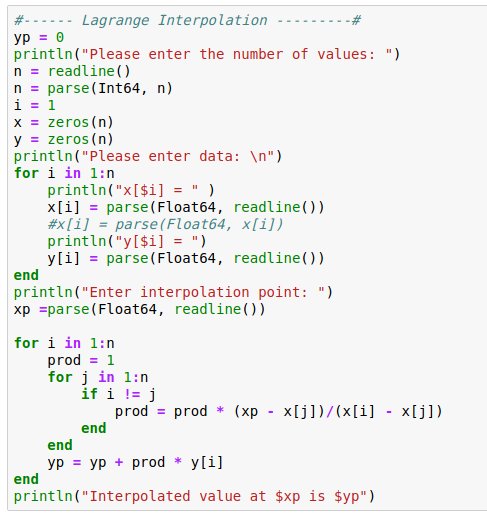
\includegraphics[width= .7\linewidth]{pic9}
		\caption{Julia code for computing Lagrange interpolation}
	\end{figure}
For the first problem running the code we have the following:
\begin{figure}[H]
	\centering
	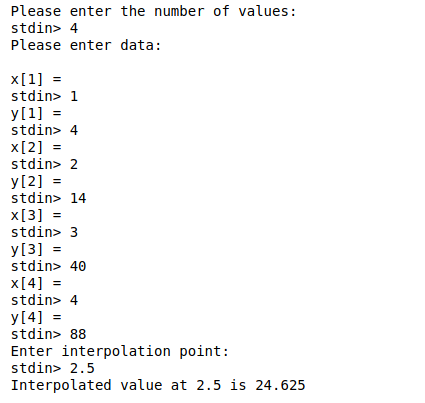
\includegraphics[width=.7\linewidth]{pic10}
\end{figure}
For the second question we have:
\begin{figure}[H]
	\centering
	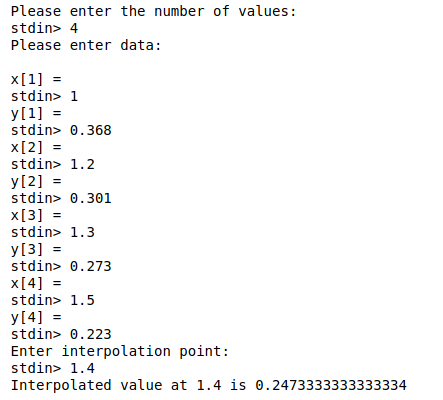
\includegraphics[width=.6\linewidth]{pic11}
\end{figure}
\end{soln}

\begin{problem}[Trapezoidal and Simpson]
	
\end{problem}
\begin{soln}
	The codes and the solutions are given in the figures below
	\begin{figure}[H]
		\centering
		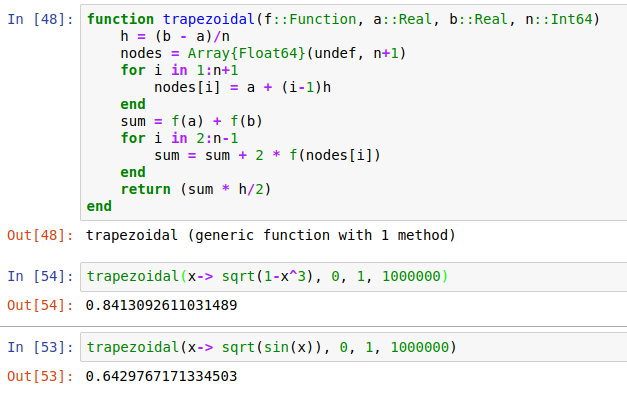
\includegraphics[width=.7\linewidth]{pic12}
		\caption{Trapezoidal rule for computing $\int_{0}^{1} \sqrt{1 - x^3} \, dx$ and $\int_{0}^{1} \sqrt{\sin x} \, dx$}
	\end{figure}

	\begin{figure}[H]
		\centering
		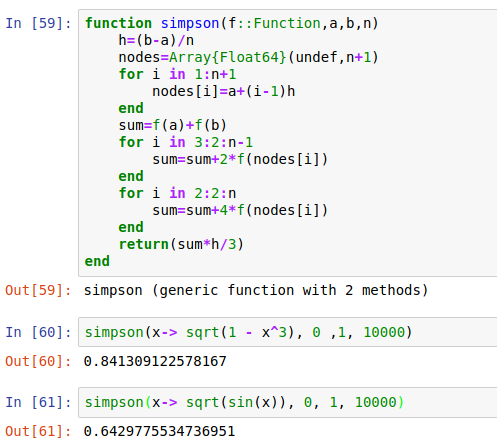
\includegraphics[width=.6\linewidth]{pic13}
		\caption{Simpson rule for computing $\int_{0}^{1} \sqrt{1 - x^3} \, dx$ and $\int_{0}^{1} \sqrt{\sin x} \, dx$}
	\end{figure}

\begin{figure}[H]
	\centering
	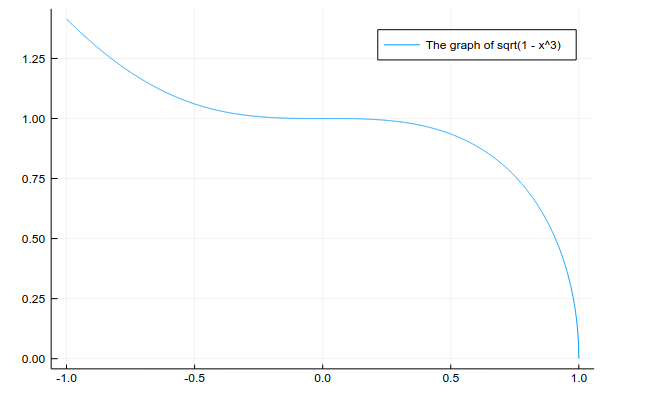
\includegraphics[width=.7\linewidth]{pic24}
	\caption{Plotting $ \sqrt{1 - x^3} \, dx$ }
\end{figure}

\begin{figure}[H]
	\centering
	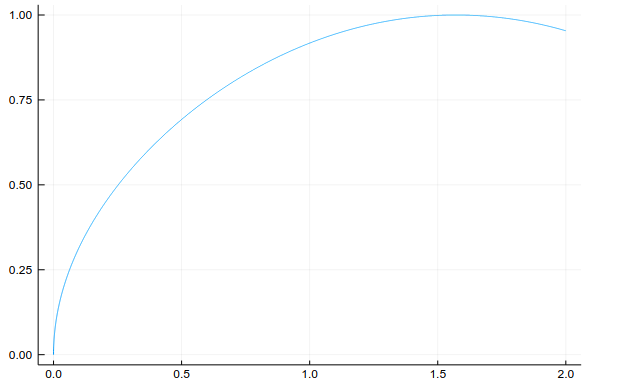
\includegraphics[width=.7\linewidth]{pic25}
	\caption{Plotting $ \sqrt{\sin x} \, dx$ }
\end{figure}



From above we can deduce that by trapezoidal rule $$\int_{0}^{1} \sqrt{1 - x^3} \, dx \approx 0.8413092611031489 \approx 0.84 $$
$$\int_{0}^{1} \sqrt{\sin x} \, dx \approx 0.6429767171334503 \approx 0.6430$$
also by Simpson rule we have $$\int_{0}^{1} \sqrt{1 - x^3} \, dx \approx 0.841309122578167 \approx 0.84 $$
$$\int_{0}^{1} \sqrt{\sin x} \, dx \approx 0.6429775534736951 \approx 0.6430$$
\end{soln}

\begin{problem}[Euler method]
	
\end{problem}
\begin{soln}
	The code for the solution of the Euler's method is given in the figure below
	\begin{figure}[H]
		\centering
		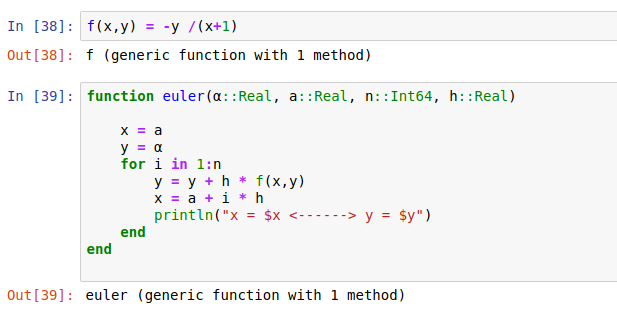
\includegraphics[width= .7\linewidth]{pic14}
		\caption{Julia code for computing $ \frac{dy}{dx} = \frac{-y}{1+x}$ using Euler's method}
	\end{figure}
To solve the given equation with $y_0 = 2, x_0 = 0.3, h= 0.1$ we have the following
\begin{figure}[H]
	\centering
	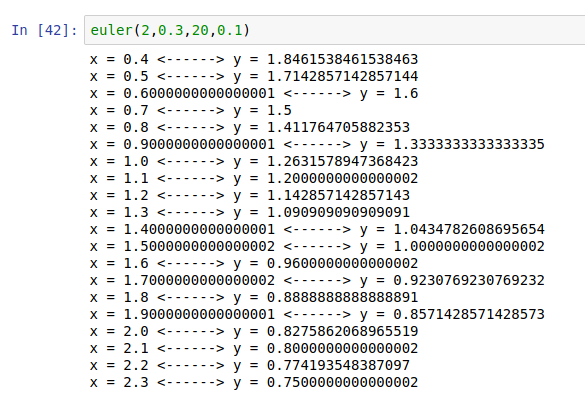
\includegraphics[width= .7\linewidth]{pic15}
	\caption{Solving $ \frac{dy}{dx} = \frac{-y}{1+x}$ using Euler's method}
\end{figure}
\begin{figure}[H]
	\centering
	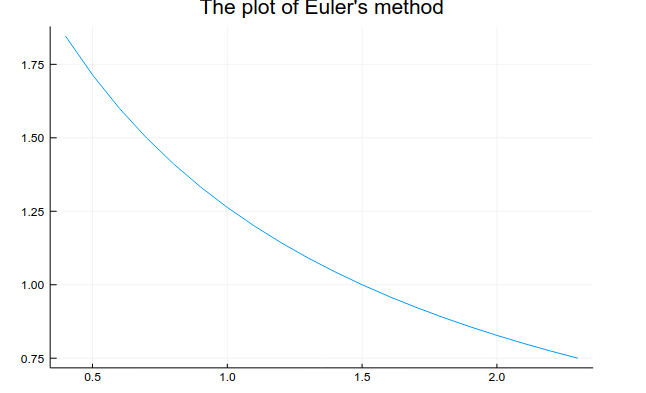
\includegraphics[width=.7\linewidth]{pic26}
	\caption{Plotting Euler method solution for $\frac{dy}{dx} = \frac{-y}{1 + x} $ }
\end{figure}
\begin{tabular}{|c|c|}
	\hline
	$x$ & $y$ \\
	\hline
	0.4 & 1.8461538461538463\\
	0.5 & 1.7142857142857144\\
	0.6 & 1.6\\
	0.7 & 1.5\\
	0.8 & 1.411764705882353\\
	0.9 & 1.3333333333333335\\
	1.0 & 1.2631578947368423\\
	1.1 & 1.2000000000000002\\
	1.2 & 1.142857142857143\\
	1.3 & 1.090909090909091\\
	1.4 & 1.0434782608695654\\
	1.5 & 1.0000000000000002\\
	1.6 & 0.9600000000000002\\
	1.7 & 0.9230769230769232\\
	1.8 & 0.8888888888888891\\
	1.9 & 0.8571428571428573\\
	2.0 & 0.8275862068965519\\
	2.1 & 0.8000000000000002\\
	2.2 & 0.774193548387097\\
	2.3 & 0.7500000000000002\\
	\hline
\end{tabular}


From the above we observe that at $x = 1, y \approx 1.2631578947368423 \approx 1.2632$

For the improved Euler's method we have the following
\begin{figure}[H]
	\centering
	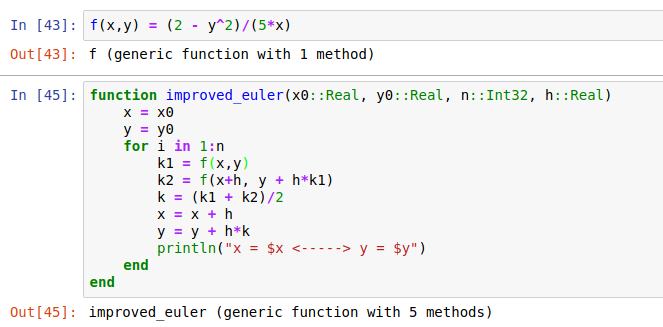
\includegraphics[width= .7\linewidth]{pic16}
	\caption{Julia code for computing $ \frac{dy}{dx} = \frac{2-y^2}{5x}$ using Euler's improved method}
\end{figure}
Solving the equation with $x_0 = 4, y_0 = 1, h = 0.2$ we have:
\begin{figure}[H]
	\centering
	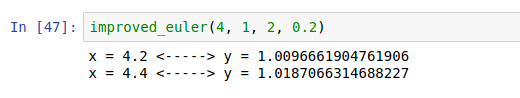
\includegraphics[width= .7\linewidth]{pic17}
	\caption{Solving $ \frac{dy}{dx} = \frac{2-y^2}{5x}$ using Euler's improved method}
\end{figure}
then we have that $ y(4.4) \approx 1.0187066314688227 \approx 1.0187$
\end{soln}

\begin{problem}[Norms]
	
\end{problem}
\begin{soln}
	Note that by definition we have 
	$$\| X\|_{2} = \left( |x_1|^2 + |x_2|^2 + \ldots + |x_n|^2 \right) ^ {\frac{1}{2}} $$
	$$\|X\|_{\infty} = \max \{ |x_1|, |x_2|, \ldots , |x_n| \} $$
	where $x_1, \ldots x_n \in X$
	
	The norm function is a predefined function in Julia, it is defined as follows for both $\| X\|_2$  and $\|X\|_\infty$ respectively
	\begin{figure}[H]
		\centering
		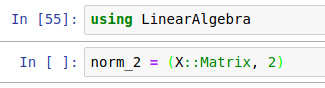
\includegraphics[width= .7\linewidth]{pic18}
		\caption{Julia code for computing $ \|X\|_2$ }
	\end{figure}
\begin{figure}[H]
	\centering
	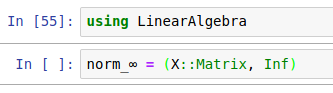
\includegraphics[width= .7\linewidth]{pic19}
	\caption{Julia code for computing $ \|X\|_\infty$ }
\end{figure}
To compute $\|X\|_2$ for $X = \left( 3,-1, 0,\frac{3}{2} \right)$ we have
\begin{figure}[H]
	\centering
	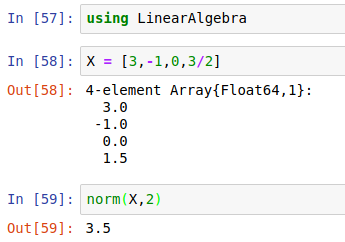
\includegraphics[width= .7\linewidth]{pic20}
	\caption{Julia code for computing $ \|X\|_2$ for $X = \left( 3,-1, 0,\frac{3}{2} \right)$}
\end{figure}
To compute $\|X\|_\infty$ for $X = \left( 3,-1, 0,\frac{3}{2} \right)$ we have
\begin{figure}[H]
	\centering
	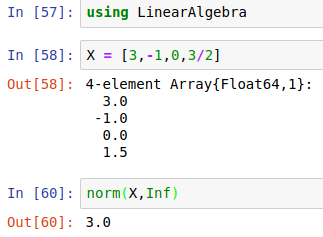
\includegraphics[width= .7\linewidth]{pic21}
	\caption{Julia code for computing $ \|X\|_\infty$ for $X = \left( 3,-1, 0,\frac{3}{2} \right)$}
\end{figure}
To compute $\| \cdot\|_\infty$ for $X = \begin{bmatrix}
10 & 15\\ 0 & 1
\end{bmatrix}$ we have the following
\begin{figure}[H]
	\centering
	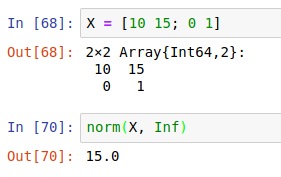
\includegraphics[width= .7\linewidth]{pic22}
	%\caption{Julia code for computing $ \|\cdot\|_\infty$ for $X = \begin{bmatrix}10 & 15 \\ 0 & 1\end{bmatrix}$}
\end{figure}

\end{soln}

\begin{thebibliography}{9}
	\bibitem{wk1} Wikipedia, \emph{Julia programming language} -- wikipedia.org/wiki/Julia\_(programming\_language)
	\bibitem{jul} \emph{Julia version 1.5.3} for Linux 
	\bibitem{jup} \emph{Jupyter Notebook for IJulia} -- Linux version 
	\bibitem{vsc} \emph{Microsoft Visual Studio Code} -- Linux version
	\bibitem{plot} \emph{Plots package for data visualization in Julia} -- Plots.jl
\end{thebibliography}

\end{document}